\documentclass[conference]{IEEEtran}
\usepackage{cite}
\usepackage{amsmath,amssymb,amsfonts}
\usepackage{algorithmic}
\usepackage{graphicx}
\usepackage{textcomp}
\usepackage{xcolor}
\def\BibTeX{{\rm B\kern-.05em{\sc i\kern-.025em b}\kern-.08em
    T\kern-.1667em\lower.7ex\hbox{E}\kern-.125emX}}
\begin{document}

\title{Multicasting in Wavelength Division Multiplexing (WDM) networks and EONs}

\author{\IEEEauthorblockN{Agnieszka Musiał}
\IEEEauthorblockA{\textit{Politechnika Wrocławska} \\
\textit{Wydział Informatyki i Telekomunikacji} \\
Wrocław, Poland \\
200910@student.pwr.edu.pl}
\and
\IEEEauthorblockN{André Carvalho}
\IEEEauthorblockA{\textit{dept. name of organization (of Aff.)} \\
\textit{name of organization (of Aff.)}\\
City, Country \\
email address}
}

\maketitle

\begin{abstract}
This paper provides literature review of multicast routing in Wavelength Division Multiplexing (WDM) networks and Elastic Optical Networks (EONs). There is a need for effective solutions in computer networks due to immense and accelerating growth of Internet traffic. WDM technology and EONs are known to increase bandwidth capacity.
\end{abstract}

\begin{IEEEkeywords}
elastic optical networks, wavelength division multiplexing, routing, multicasting
\end{IEEEkeywords}

\section{Introduction}

\subsection{Multicasting}
Multicasting is a type of routing scheme in a network, where data is transferred from root node to selected receiving nodes.

In multicast data is propagated over minimum Steiner tree or minimum spanning tree of all recipients, so that it is sent over each link exactly once. It is more efficient than unicasting to selected nodes. Even though unicast also adopts minimum Steiner tree or minimum spanning tree, paths are calculated separately between root and each receiving node. It is likely that data would be sent over same link multiple times, if that link exists in many calculated paths.

Therefore multicast requires less traffic than unicast.

\subsection{Wavelength division multiplexing}
Wavelength division multiplexing (WDM) is physical technology, that increases capacity of optical fiber by using electromagnetic properties of light.

In fibre-optic communication carrier of data is light, which is an electromagnetic wave with inversely proportional properties of wavelength and frequency. Light of different wavelengths can be multiplexed together, creating complex signal that can be transferred over single optical fibre. At the receiving end signal is demultiplexed back into many signals and each is provided to corresponding recipients.

Following are types of WDM systems:
\begin{itemize}
	\item normal (WDM), wavelengths 1310 nm and 1550 nm on one fiber.
	\item coarse (CWDM), wavelengths 1271 nm to 1611 nm with channel spacing 20 nm.
	\item dense (DWDM), wavelengths 1530 nm to 1565 nm with channel spacing 0.8/0.4 nm.
\end{itemize}

A substantial component of WDM are thin-film filters. They can pass certain wavelengths and reflect all other wavelengths. In WDM demultiplexer they are positioned in a cascade form, easily efficiently extracting original signals. Exemplary design of such system is presented on figure  \ref{demultiplexing}.

\begin{figure}[htbp]
	\centerline{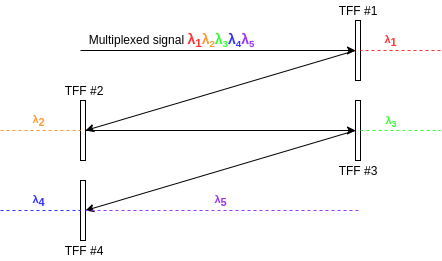
\includegraphics[scale=0.5]{demultiplexer.png}}
	\caption{Demultiplexing in WDM}
	\label{demultiplexing}
\end{figure}

\subsection{EONs}
Elastic optical network (EON) is a novel approach to optical networks. 

\section{Multicasting in WDM}

\section{Multicasting in EONs}

\begin{thebibliography}{00}
\bibitem{b1}
\end{thebibliography}
\end{document}
